
%(BEGIN_QUESTION)
% Copyright 2010, Tony R. Kuphaldt, released under the Creative Commons Attribution License (v 1.0)
% This means you may do almost anything with this work of mine, so long as you give me proper credit

Suppose an instrument technician needs to perform service and testing on a control valve while the process is still operating (flow still going through the pipes).  An operator comes over to the control valve to ``block and bypass'' it for the technician so that the technician will be able to stroke the valve freely without affecting the process.  The operator's goal is to achieve the exact same rate of fluid flow through the bypass valve that is now flowing through the control valve, so that both block valves may be shut and the technician given freedom to do anything to the control valve:

$$\includegraphics[width=15.5cm]{i04354x01.eps}$$

The operator's first step is to begin opening the bypass valve while leaving the flow controller (FIC) in automatic mode.  Identify whether the operator needs to watch the flow indicator (FI) while opening the bypass valve, or watch the control valve stem position while opening the bypass valve, in order to determine the proper amount of opening for the bypass valve before closing both block valves.  Furthermore, identify precisely what the operator should be looking for while watching, in order to know when he or she has reached the proper bypass valve position.

\underbar{file i04354}
%(END_QUESTION)





%(BEGIN_ANSWER)

If the operator watches the control valve stem position, he or she needs to stop opening the bypass valve as soon as the control valve reaches the full-closed position under automatic control.

\vskip 10pt

If the operator watches the flow indicator, he or she needs to stop opening the bypass valve as soon as the indicator registers a flow rate above setpoint that does not recover back to setpoint after a short time.

%(END_ANSWER)





%(BEGIN_NOTES)


%INDEX% Final Control Elements, valve: performing maintenance on live system

%(END_NOTES)


